\chapter{Implementazione}
\label{implementazione}
In questa sezione è descritta l'implementazione del progetto definito nel capitolo precedente. I principali strumenti utilizzati sono Python come linguaggio di programmazione e le librerie Scikit-learn \cite{sklearn} per attuare machine learning e Keras \cite{keras} per realizzare reti neurali. La libreria per reti neurali su cui opera Keras è Tensorflow \cite{tensorflow}.
Di seguito sono elencati i dettagli implementativi delle singole entità, ed i parametri usati durante la fase sperimentale.

\section{Classificatore Random Forest}
\label{imp:randomforest}
Il classificatore Random Forest è stato implementato tramite l'uso della libreria python Scikit-learn \cite{sklearn}. 
Al fine di avere un ambiente di testing facilmente fruibile, è stata creata una classe $MyClassifier$ in grado di gestire la serie di esperimenti effettuata sul classificatore. Tali esperimenti hanno permesso di testare i differenti parametri di funzionamento e la composizione delle features che compongo il dataset del classificatore. In figura \ref{fig:uml_randomforest} è mostrata la struttura della classe $MyClassifier$, la quale contiene le funzioni principali di inizializzazione, salvataggio e caricamento dei parametri, salvataggio e caricamento dei risultati oltre che alle funzioni necessarie per allenare il classificatore (funzione $fit$), eseguire cross-validation (funzione $cross\_validate$), produrre grafici di risultati ($classification\_report$ e $plot_AUC$) ed eseguire predizione su di una lista di domini in input (a fini di testing).

\begin{figure}[!htb]
	\centering
	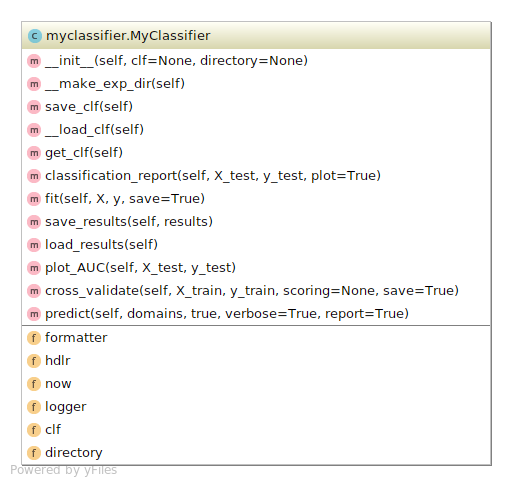
\includegraphics[width=0.7\columnwidth]{figures/uml_randomforest.png}
	\caption{Diagramma UML della classe MyClassifier 			\label{fig:uml_randomforest}}
\end{figure}


\subsection{Dataset}
Il dataset utilizzato per le fasi di training e testing del classificatore è stato definito nella sezione \ref{pro:randomforestdataset}. A livello operativo il dataset è stato generato a partire dai soli nomi di dominio in formato stringa, per i quali sono stati estratti le singole features. Segue una descrizione dettagliata delle features utilizzate per generare il dataset.

\begin{itemize}
\item \textbf{MCRExtractor} si occupa di fornire il rapporto tra caratteri significativi. \`E caratterizzato dal parametro che identifica la minima sottostringa da analizzare, composta da 3 caratteri. L'algoritmo cicla per ogni dimensione di n-gramma $\geq 3$ , estrae le tuple di dimensione $i$ dalla stringa e per ogni tupla $s$ presente in una $word$ del dizionario inglese, viene aggiunta la sua lunghezza alla somma dei caratteri significativi della stringa. 
Il risultato è il rapporto tra la somma della lunghezza dei caratteri significativi e la lunghezza totale della stringa.
 
\begin{lstlisting}[language=Python]
min_subtr = 3
maxl = 0
for i in range(min_subtr, len(str(domain_name))):
	tuples = zip(*[str(domain_name)[j::i] for j in range(i)])
	split = [''.join(t) for t in tuples]
	tmpsum = 0
	tmps = []
	for s in split:
		for words in eng_dict:
			if s in words:
				tmpsum += len(s)
				tmps.append(s)

	if tmpsum > maxl:
		maxl = tmpsum
return maxl / int(len(str(domain_name)))
\end{lstlisting}

\item \textbf{NormalityScoreExtractor} estrae il punteggio di normalità degli n-grammi. A differenza del lavoro propsoto in \cite{Schiavoni2014}, si è scelto di estrarre il \textit{normality score} per gli n-grammi di lunghezza 1,2,3,4,5 caratteri, in quanto in fase sperimentale hanno dimostrato di fornire un apporto significativo alla precisione del classificatore. \`E definito dal seguente algoritmo, dove il valore $self.n$ identifica la lunghezza dell'n-gramma da valutare. L'algoritmo separa in n-grammi di dimensione $n$ la stringa e per ogni tupla di caratteri $s$, somma il numero di occorrenze di tale tupla all'interno del vocabolario inglese, ritornando il rapporto tra il valore complessivo delle occorenze delle tuple nel vocabolario inglese e la lunghezza della stringa meno $n+1$.

\begin{lstlisting}[language=Python]
if len(str(domain_name)) < self.n:
            return 0
tuples = ngrams(str(domain_name), self.n)
myngrams = (''.join(t) for t in tuples)
scoresum = 0
for s in myngrams:
	counter = 0
    for words in eng_dict:
    	if s in words:
        	counter += 1
    scoresum += counter
return scoresum / (len(str(domain_name)) - self.n + 1)
\end{lstlisting}

\item \textbf{NumCharRatio} estrae il rapporto di caratteri numerici rispetto alla lunghezza della stringa

\begin{lstlisting}[language=Python]
counter = Counter(domain_name)
ncr = 0
for key, value in counter.iteritems():
	if key.isdigit():
		ncr += value

return ncr / len(domain_name)
\end{lstlisting}

\item \textbf{DomainNameLength} estrae la lunghezza del nome di dominio.

\begin{lstlisting}[language=Python]
return (len(domain_name))
\end{lstlisting}

\item \textbf{VowelConsonantRatio} estrae il rapporto tra vocali e consonanti all'interno della stringa.

\begin{lstlisting}[language=Python]
count = 0
vowels = set("aeiou")
for letter in domain_name:
	if letter in vowels:
		count += 1
return count / (len(domain_name) - count)
\end{lstlisting}

\end{itemize}

L'insieme di tali features è stato usato per generare un dataset contenente per ogni nome di dominio le 9 features linguistiche generate a partire dalle stringhe dei nomi di dominio. 

Assieme a tale dataset è stato generato un vettore binario "\textit{target}" da cui il classificatore può verificare la categoria di appartenenza (malevolo o reale) di ogni dominio.

\subsection{Ambiente di training}
Durante la fase di training il dataset è stato mescolato e separato in due subset: \textit{train} e \textit{test}. Il subset di testing ha la dimensione pari al 10\% dell'intero dataset. 

La fase di training è stata eseguita tramite la tecnica di convalida incrociata (\textit{k-fold cross validation}) in cui il dataset di training è stato separato in 10 subset (\textit{fold)} e ad ogni passo la \textit{k-esima} parte è stata usata come validazione per la fase di training. Questa tecnica evita il problema dell'overfitting, di cui generalmente soffrono i modelli di machine learning.

Il restante subset di test, mai applicato nella fase di training, è stato utilizzato per valutare il modello del classificatore.


\subsection{Parametri Classificatore}
In particolare i parametri del classificatore utilizzato che sono stati modificati dal loro valore di default sono:
\begin{itemize}
\item \textbf{\texttt{n\_estimators}} = 100. Numero di stimatori da utilizzare nel processo. Il valore è stato deciso come ottimale dopo una serie di test sperimentali preliminari.
\item \textbf{\texttt{min\_samples\_leaf}} = 50. Numero minimo di campioni per un nodo foglia. il valore è stato deciso come ottimale dopo una serie di test sperimentali preliminari.
\item \textbf{\texttt{oob\_score}} = True. Implica l'uso di campioni \textit{out-of-bag} per ottenere una stima facilitata dell'errore. Con questa tecnica una parte del campione di stima viene esclusa per essere utilizzata come insieme di verifica.
\end{itemize}

\section{Classificatore Neurale}
\label{imp:classneurale}
L'implementazione del classificatore neurale è stata eseguita in ambiente Python, con l'utilizzo della libreria Keras \cite{keras} per le reti neurali.
Per motivi di semplicità si è scelto di copiare l'ambiente di testing definito per il classificatore Random Forest mostrato in figura  \ref{fig:uml_randomforest}. Tale classe permette di gestire i diversi esperimenti, utilizzati per decidere quale composizione del \textit{Multi Layer Perceptron}  (abbr. MLP) in base ai risultati sperimentali. 
Il punto saliente del classificatore è formato dalla sua baseline, la quale contiene i livelli che effettivamente compongono la rete neurale.

\subsection{Baseline}
Come definito all'interno della sezione \ref{classificatorenninterno}, la composizione del MLP è stata decisa dopo un confronto tra tre modelli differenti nella conformazione: 

\begin{itemize}
\item un primo modello ridotto contenente un input a dimensione 15 (fissata inizialmente come dimensione dei domini codificati), un livello intermedio di dimensione dimezzata rispetto all'input ed un livello finale con un singolo neurone per ottenere classificazione binaria (listato \ref{lst:small} ). 


\lstinputlisting[language={}, caption={Baseline Ridotta},label={lst:small}]{code/small_baseline.log}


\item un secondo modello ampliato contenente input equivalente al precedente, due livelli interni di dimensione 128 ed una uscita con singolo neurone. (listato \ref{lst:large} ).


\lstinputlisting[language={}, caption={Baseline ampliata},label={lst:large}]{code/large_baseline.log}


\item un modello intermedio, contenente ingresso equivalente al precedente, due livelli interni da 128 e 64 e uscita con singolo neurone. (listato \ref{lst:pieraz}).


\lstinputlisting[language={}, caption={Baseline intermedia.},label={lst:pieraz}]{code/pieraz_baseline.log}

\end{itemize}

Tutti i modelli contengono al loro interno oltre che i dense layer, dei layer aggiuntivi per ottimizzare la fase di training, in particolare i layer Dropout e Batch Normalization per contrastare il fenomeno dell'\textit{overfitting}. Dopo una fase sperimentale si è deciso di optare per il modello intermedio, in quanto ha espresso i risultati migliori a fronte di un ridotto consumo di risorse.

\subsection{Dataset}
Come definito all'interno della sezione \ref{classificatorenninput} il dataset utilizzato per il classificatore neurale è differente dal caso precedente in quanto i domini vengono codificati in forma di vettori numerici, mappati rispetto ad un dizionario di caratteri ammissibili per i domini di rete (tabella \ref{tab:dict}).

\begin{table}[!ht]
    \centering
    \begin{tabular}[t]{ll}
    \toprule
    Key & Value \\
    \midrule
1 & a \\
2 & b \\
3 & c \\
4 & d \\
5 & e \\
6 & f \\
7 & g \\
8 & h \\
9 & i \\
10 & j \\
\bottomrule        

\end{tabular}
\begin{tabular}[t]{ll}
    \toprule
    Key & Value \\
    \midrule
11 & k \\
12 & l \\
13 & m \\
14 & n \\
15 & o \\
16 & p \\
17 & q \\
18 & r \\
19 & s \\
20 & t \\
\bottomrule        
\end{tabular}
\begin{tabular}[t]{ll}
    \toprule
    Key & Value \\
    \midrule
21 & u \\
22 & v \\
23 & w \\
24 & x \\
25 & y \\
26 & z \\
27 & 0 \\
28 & 1 \\
29 & 2 \\
30 & 3 \\
\bottomrule        
\end{tabular}
\begin{tabular}[t]{ll}
    \toprule
    Key & Value \\
    \midrule
31 & 4 \\
32 & 5 \\
33 & 6 \\
34 & 7 \\
35 & 8 \\
36 & 9 \\
37 & - \\
38 & . \\
\bottomrule        
    \end{tabular}
    \caption{Dizionaro di caratteri mappati. \label{tab:dict}}
\end{table}

Tale mapping permette al MLP di estrarre features a partire dai caratteri che compongono i domini.

\subsection{Ottimizzatore}
I modelli testati in questa sezione sono stati compilati utilizzando l'ottimizzatore \textit{Adaptive Moment Estimation (abbr. adam)} \cite{adam}. Tale ottimizzatore fornisce generalmente le prestazioni migliori nel caso di classificazione binaria e pertanto si è optati per tale soluzione.

\subsection{Fase di Training}
Durante la fase di training si sono testati gli iperparametri principali che pilotano la performance del classificatore: in particolare i valori della dimensione del tensore di ingresso  \lstinline!batch_size! ed il numero di epoche \lstinline!epochs! sul quale eseguire la fase di training.

Dopo una fase sperimentale i valori che hanno mostrato i risultati migliori in fase di valutazione sono stati: 
\begin{itemize}
\item \textbf{batch\_size} = 35 
\item \textbf{epochs} = 60
\end{itemize}

\section{Autoencoder}
\label{imp:autoencoder}
L'implementazione dell'autoencoder descritto in sezione \ref{autoencoder} è stata eseguita in ambiente Python con l'ausilio della libreria Keras per reti neurali. 

\subsection{Dataset}
Il dataset utilizzato per il training dell'autoencoder è stato definito nella sezione \ref{datasetautoencoder}. Tale dataset risulta essere un'ulteriore elaborazione della mappatura utilizzata all'interno del classificatore neurale precedentemente descritto: i domini codificati in vettori numerici sono stati ulteriormente codificati con la tecnica one-hot, in modo da ottenere, per ogni dominio, un tensore di valori binari contenente un vettore per ogni \textit{step temporale} che compone il dominio. tale vettore, contenente la lettera i-esima del dizionario è formato da zeri tranne l'elemento alla posizione i-esima, impostato ad 1.

Questa ulteriore codifica ha permesso successivamente di poter trasformare l'autoencoder in una GAN, inviando l'output del decoder come input dell'encoder senza effettuare operazioni di campionamento, fonte di rottura del gradiente del modello.

La differenza principale con il dataset usato precedentemente per il classificatore neurale è la totale mancanza di domini DGA e l'uso esclusivo di domini forniti dal database di Alexa \cite{amazon:alexa}. Il fine infatti è ottenere un sistema che possa riprodurre al meglio i domini reali.


\subsection{Encoder}
La struttura dell'Encoder, definita all'interno della sezione \ref{encoder} è stata implementata con l'ausilio delle API funzionali fornite da Keras. In questo modo è stato possibile implementare un modello più complesso del precedente classificatore, in grado di eseguire l'operazione convoluzionale con due diverse conformazioni in contemporanea rispetto allo stesso tensore di ingresso. Di seguito sono mostrati gli iperparametri che definiscono il modello Encoder. 

\lstinputlisting[caption={Iperarametri Encoder.},label={lst:par_enc},lastline=9]{code/encoder.py}

\`E possibile notare quali parametri definiscono le due reti convoluzionali:
\begin{itemize}
\item Convnet formata da 20 filtri, kernel di dimensione 2 e passo 1.
\item Convnet formata da 10 filtri, kernel di dimensione 3 e passo 1.
\end{itemize}

La bontà di tali valori è stata confermata da \cite{deepdga} e per tanto utilizzati in maniera identica.
I valori \lstinline!timesteps!, \lstinline!word_index!, \lstinline!latent_vector! definiscono le dimensioni dei tensori di ingresso ed uscita, così come definiti dalle dimensioni del dataset. La dimensione di \lstinline!latent_vector! è arbitraria: in questo caso si è optato per  ridurre ulteriormente la dimensione del tensore di uscita dalle due reti convoluzionali per estrarre le features più caratterizzanti dalla fase di encoding.

I valori \lstinline!dropout_value! e \lstinline!leaky_relu_alpha! sono il risultato di una lunga fase di \textit{tuning} degli iperparametri, particolarmente critici per il mantenimento dell'equilibrio della successiva GAN.

Per completezza di seguito è elencato il codice essenziale che compone l'encoder.

\lstinputlisting[caption={Struttura livelli Encoder.},label={lst:str_enc},firstline=9]{code/encoder.py}

\subsection{Decoder}
La composizione del decoder è pressochè identica a quella mostrata dall'encoder e ricalca il progetto mostrato in sezione \ref{decoder}. Di seguito sono elencati gli iperparametri che compongono il modello decoder. Si può notare come siano identici a quelli mostrati dall'encoder a differenza del \lstinline!dropout_value!, il quale gioca un ruolo maggiore nel pilotare l'equilibrio tra i due modelli.

\lstinputlisting[caption={Iperarametri Decoder.},label={lst:par_enc},lastline=10]{code/decoder.py}

Per completezza si riporta l'implementazione del decoder:

\lstinputlisting[caption={Struttura livelli Decoder.},label={lst:str_enc},firstline=10]{code/decoder.py}

\subsection{Training}
Durante la fase di training si è realizzato il modello generale che compone l'autoencoder, sottoforma di modello sequenziale Keras \lstinline!keras.models.Sequential!. Tale modello è composto da due livelli: Encoder e Decoder
Il modello è compilato con l'uso dell'ottimizzatore \textit{adam} e \textit{Categorical Cross Entropy} come funzione di \textit{loss}. Tale scelta è dovuta alla natura dell'autoencoder, al quale viene dato come target per il training lo stesso dataset da input al fine di mimare il più correttamente possibile l'input iniziale passando per una codifica a minore dimensione.

\lstinputlisting[language={},basicstyle=\ttfamily\footnotesize,caption={Composizione di massima dell'autoencoder},label={lst:aenc}]{code/autoencoder.log}

I valori di \lstinline!batch_size! ed \lstinline!epochs! sono stati definiti tali dopo una breve fase sperimentale:
\begin{itemize}
\item \textbf{batch\_size} = 128 
\item \textbf{epochs} = 200
\end{itemize}

Durante la fase di training l'indicatore principale di performance è il valore di \textit{loss}, il quale al suo decrescere indica una migliore capacità di riproduzione dei domini.

\section{Generative Adversarial Network}
\label{imp:gan}
L'implementazione della Generative Adversarial Network (sezione \ref{ganintro}, è stata evoluta a partire da quella eseguita per l'autoencoder. 

\subsection{Dataset}
La composizione del dataset di domini è identica a quella fornita per l'autoencoder. Durante la fase di training si alternano mini-batch provenienti da tale dataset e mini-batch create sinteticamente dal generatore a partire da un vettore randomico di valori compresi tra $[-1.0,1.0]$.

\subsection{Discriminatore}
Il modello del discriminatore è derivato dal modello definito dall'encoder: in coda all'encoder si è aggiunto un layer denso in grado di operare classificazione binaria, definito da: 

\begin{lstlisting}
Dense(1, activation='sigmoid', kernel_initializer='normal')
\end{lstlisting}

Questo layer aggiuntivo trasforma la funzione dell'encoder in un classificatore in grado di discriminare tra domini reali e domini generati sinteticamente.

\subsection{Generatore}
La struttura del generatore è identica alla struttura definita per il decoder. La differenza principale sta nel tipo di input dato in ingresso: Nel caso decoder l'input proviene dall'uscita dell'encoder, mentre nel caso generatore l'input è fornito in forma di vettore randomico creato con l'ausilio della libreria \textit{numpy} \cite{numpy} \lstinline!np.random.normal! con valori compresi tra $[-1.0,1.0]$.

\subsection{Training}
La fase di training comporta più fasi, che coinvolgono separatamente i sottosistemi della GAN.

In prima fase, come indicato da \cite{deepdga} si è scelto di eseguire un pre-training tramite l'autoencoder. Si è eseguita una fase di training efficace su tale sistema, copiando successivamente i pesi aggiornati all'interno della GAN, al fine di fornire una base di partenza stabile per entrambi i sottosistemi Encoder/Discriminatore e Decoder/Generatore.

Successivamente a tale pre-training il dataset viene caricato in memoria, i modelli di Discriminatore e Generatore sono compilati con i seguenti valori: 
\begin{itemize}
	\item \textbf{Discriminatore}: utilizza l'ottimizzatore RMSprop \cite{rmsprop} con tali valori: 
		\begin{itemize}
			\item learning rate $= 0.01$ 
			\item clipvalue $= 1.0$
			\item decay $= 10^{-8}$
		\end{itemize}
	\item \textbf{Generatore}: utilizza l'ottimizzatore Adam con tali valori:
	\begin{itemize}
		\item learning rate $= 0.0001$
		\item beta\_1 $= 0.9$
		\item beta\_2 $= 0.999$
		\item $\epsilon = 10^{-8}$
		\item decay $= 10^{-8}$
		\item clipvalue  $= 1.0$
	\end{itemize}
\end{itemize}

Tali valori sono il frutto di una fase sperimentale molto lunga, durante la quale si è cercato di calibrare attentamente i valori di learning rate di entrambi gli ottimizzatori al fine di ottenere un equilibrio tra i due sottosistemi della GAN: ha infatti dimostrato una forte propensione a degenerare verso un sistema o l'altro, fornendo valori di loss estremi. Si è cercata infatti una impostazione tale che mantenesse valori di loss più o meno stabili durante la durata della fase di training.

Entrambi i sottosistemi sono stati compilati con l'uso di \textit{binary crossentropy} come funzione di loss, in quanto l'output di entrambi è rappresentato dal layer denso, in uscita dal discriminatore.

Nella fase successiva il dataset è stato suddiviso secondo la dimensione impostata dal valore di \lstinline!batch_size!, in modo da poter garantire una passata completa a tutto il dataset per ogni epoca di training.
Per ogni epoca e per ogni minibatch del dataset si è proceduto con il seguente metodo: 
\begin{itemize}
	\item Si genera un vettore di valori randomici, di dimensione identica all'input accettato dal Generatore. 
	\item A partire da tale vettore si sono generati domini sintetici.
	\item In maniera alternata, per ogni ciclo di mini-batch, si è fornito come training al discriminatore un mini-batch formato unicamente da domini reali provenienti dal dataset oppure un mini-batch di domini sintetici prodotti dal generatore. Entrambi gli input sono accompagnati da un vettore di target che indica al discriminatore la natura di tali domini (reali o sintetici).
	\item Si congelano i pesi del discriminatore. Tale procedura permette al generatore di procedere alla sua fase di training, utilizzando il discriminatore come mezzo per ottenere un indice di qualità dei domini generati sinteticamente.
	\item Si genera un nuovo vettore randomico.
	\item Si procede al training del generatore, utilizzando l'intera GAN come modello. In ingresso si forniscono il vettore randomico ed un vettore di target ingannevole, il quale indica che i valori in uscita forniti sono reali. Questo metodo fa si che il generatore si spinga via via verso la creazione di domini via via più simili a quelli reali. L'output del generatore viene dato in ingresso al livello successivo, composto dal discriminatore che in questo caso non può aggiornare i propri pesi ma solo fornire una predizione sulla natura dei dati di ingresso. 
	\item Si riattiva l'aggiornamento dei pesi per il discriminatore, per il prossimo ciclo di training.
\end{itemize}

Tale procedura è ripetuta per tutti i mini-batch e per il numero di epoche di training impostato. 